\documentclass[conference]{IEEEtran}
\IEEEoverridecommandlockouts
% The preceding line is only needed to identify funding in the first footnote. If that is unneeded, please comment it out.
\usepackage{cite}
\usepackage{amsmath,amssymb,amsfonts}
\usepackage{algorithmic}
\usepackage{graphicx}
\usepackage{textcomp}
\usepackage{xspace}
\usepackage{url}
\def\BibTeX{{\rm B\kern-.05em{\sc i\kern-.025em b}\kern-.08em
    T\kern-.1667em\lower.7ex\hbox{E}\kern-.125emX}}
    
% Put edit comments in a really ugly standout display
\usepackage{times} 
 
\newcommand{\todo}[1]{\textbf{\textcolor{red}{TODO: #1}}} 
% Macros for proof-reading & corrections
\usepackage[normalem]{ulem} % for \sout  
\usepackage{xcolor}  

\usepackage{ifthen}
\usepackage{amssymb} 

\usepackage{backnaur}
  
\newboolean{showcomments}
\setboolean{showcomments}{true} % toggle to show or hide comments
\ifthenelse{\boolean{showcomments}}     
  {\newcommand{\nb}[2]{   
    \fcolorbox{gray}{yellow}{\bfseries\sffamily\scriptsize#1}
    {$\blacktriangleright$#2$\blacktriangleleft$}
   }
   \newcommand{\version}{\emph{\scriptsize$-$working$-$}}  
  }
  {\newcommand{\nb}[2]{} 
   \newcommand{\version}{} 
  } 

\newcommand\levi[1]{\nb{Levi}{\textcolor{teal}{#1}}} 
\newcommand\sudeep[1]{\nb{Saad}{\textcolor{teal}{#1}}} 

\newcommand{\ears}{\textsc{Ears}\xspace}
\newcommand{\etal}{\emph{et al.}\xspace}
\newcommand{\earsctrl}{\textsc{Ears-Ctrl}\xspace}
\newcommand{\ltl}{\textsc{Ltl}\xspace}
\newcommand{\iets}{\textsc{Iets3}\xspace}
\newcommand{\fig}{figure\xspace} 

\newtheorem{definition}{Definition} 

\begin{document} 
  
\title{Formalizing EARS} 
% {\footnotesize \textsuperscript{*}Note: Sub-titles are not captured in Xplore and
% should not be used}
% \thanks{Identify applicable funding agency here. If none, delete this.}
 
\author{\IEEEauthorblockN{Levi L\'ucio, Saad Bin Abid, Tahira Iqbal }
\IEEEauthorblockA{\textit{fortiss GmbH} \\  
\textit{Guerickestrasse 25}\\
Munich, Germany \\ 
\{lucio, abid, iqbal\}@fortiss.org  
} 

}

\maketitle 


\begin{abstract} 
The Easy Approach to Requirements Specification (\ears) has been designed
primarily as a set of templates to assist requirements engineers in writing
software requirements that are clear and understandable.
Its target are thus requirements engineers, software architects and developers.
Due to the minimalistic nature of the English sentences that make up an \ears
specification, it is reasonable to expect that automated tasks can be performed
on \ears specification, among which verification and code synthesis. Given
English cannot be directly understood by machines without some degree of
ambiguity, \ears requirements can only by automatically processed if they are
translated in advance into formal specifications. In this short paper, we
explore how a translation from \ears into Linear Temporal Logic can be
implemented in practice. 
\end{abstract} 

\section{Introduction and Problem Statement}

\ears~\cite{EARS09} has been designed at Rolls-Royce having in mind helping
requirements engineers to specify requirements that are as unambiguous, complete
and objective as possible -- while being written in natural language.
Technically architecting and writing software is an expensive task.
Misunderstandings in communicating requirements to architects and developers
amount to using precious software development resources in an unfruitful manner,
leading to project overbudgeting and/or failure~\cite{chaos:2014}. Mavin \etal
have shown with their work that, by using a simple set of template english
sentences for specifying requirements, ambiguity, partiality and subjectivity
can be significantly reduced in textual requirements, even for large
specifications~\cite{EARS10,EARS16}.

A byproduct of having requirements written in a simple subset of natural
language is that automation becomes more possible. The regularity of \ears lends
itself well to mathematical treatment and, given the wealth of research in
formal methods, it is only reasonable to investigate how \ears specifications
can be turned into fully precise formal specifications. Such formal
specifications can then be used for purposes such as \emph{code synthesis},
\emph{formal verification} or \emph{test generation}.

The work we present here is motivated by the \iets project\footnote{IETS3 was
funded by the German Federal Ministry of Education and Research under code
01IS15037A/B} ran recently by our company on the construction of languages for
requirements engineering. With \iets we have been able to synthesise code
directly from \ears specifications. To that end, we have transformed \ears into
Linear Temporal Logic (\ltl), a mathematical formalism that allows expressing
temporal dependencies between the states of a system. This transformation is
part of the \earsctrl environment~\cite{earsctrlProcess} that allows
synthesizing code directly from requirements expressed in
\ears~\cite{LucioRCA16,LucioRAM17}.

In this paper we will elaborate on how this translation has been implemented,
indentify some of the hurdles found when building such a translation and
extrapolate some of our lessons learned into the bigger picture of having a
formal couterpart to \ears. 
 
\section{Formalizing EARS using Linear Temporal Logic}

In this section we will use as running example the simplified requirements for
a controller for the engines of a (unspecified) machine. The machine includes a
\emph{main}, an \emph{auxiliary} and an \emph{oil pump} engine. The sequence to
start the machine is to first run the old pump engine; after 10 seconds start
the main engine; and finally after 5 more seconds start the auxiliary engine.
The \ears requirements for such a controller are depicted in
\fig\ref{fig:reqs_motor}.

\begin{figure}[!h]
\centering
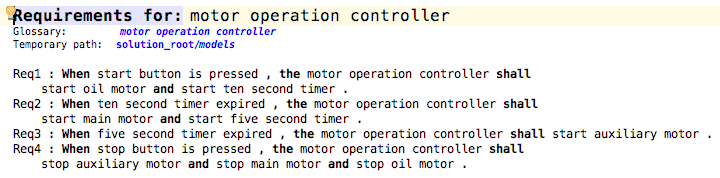
\includegraphics[width=.5\textwidth]{figures/motor_ears}
\caption{\ears requirements expressed in the \earsctrl tool}
\label{fig:reqs_motor}
\end{figure}

Let us now build a set of \ltl formulas that reflect the semantics of these
requirements. \ltl builds on propositional logic by adding temporal operators to
it. Formulas in \ltl are particularly appropriate to express properties of
runs of a reactive system, meaning how the state of that system should evolve
over time. For example, one may want to state that always when a motor is on,
then a thermostat is measuring its temperature. Or that, while the start button
is pressed then the starter engine will attempt to run the main engine. Or
even, that eventually the motor will stop. \ltl incorporates operators to
describe these situations. Due to space limitations we will not
formally introduce \ltl here, but will rather explain the formulas that we
introduce via our running example.

By looking carefully at the example in \fig\ref{fig:reqs_motor} it is possible
to understand that all requirements are given in the form of \ears event-driven
templates. Take for instance Req1. The translation of Req1 into \ltl would be as
follows:

\begin{multline}
\mathbf{G}(start_button_pressed \rightarrow\\ \textbf{X}(som\land
stst))
\end{multline}



\begin{itemize}
  \item A specification of a motor controller in EARS-CTRL
  \item Simple introduction to LTL
  \item Naive transformation of the motor requirements into LTL
\end{itemize}

\section{The Importance of Context}
\label{sec:context}

While the translation we have presented in \sect\ref{sec:formalization}
provides a boilerplate to transform \ears into \ltl, the rules given in
\tab\ref{fig:translation_ears_ltl} are naive regarding the interaction between
the complete set of requirements in an \ears specification. For example, if one
take into consideration the transformation rule for \emph{Event-Driven} requirements, the \ltl formlula
corresponding to those will only state that in the moment immediately after the
\emph{trigger} is received, the \emph{response} will be given. However,
the requirement states nothing about the life of the system after
that moment. It is reasonable to ask questions such as:

\begin{enumerate}
  \item after a \emph{trigger} is received, will the \emph{response}
  keep produced by the system for some period?
  \label{q1}
  \item if so, until when?
  \label{q2}
\end{enumerate}

While it is challenging to come up with a generic answer for these questions,
we will attempt to describe a solution for the case in which such a specification is
used for code synthesis, as is done in our \earsctrl tool.

As mentioned in \sect\ref{sec:introduction}, \earsctrl was built to synthesize
software controllers directly from requirements written in \ears. Software
controllers receive input from \emph{sensors} and produce output on
\emph{actuators}. By orchestrating those signals a software controller
controls the operation of a machine, such as the system of motors presented in
\fig\ref{fig:reqs_motor}.

Coming back to questions \ref{q1} and \ref{q2} above, let us attempt to answer
then by analysing a concrete example based on our motor controller case study.
Part of \textsf{Req1} states that when the \emph{start button} is pressed then
the \emph{oil motor} will start. It is assumed that the motor will continue to
be on until it is shutdown\footnote{Note that we assume that $\text{\emph{start
motor oil}} = \neg(\text{\emph{stop motor oil}})$. In \earsctrl this is
explicitely expressed in a glossary accompanying the requirements in
\fig\ref{fig:reqs_motor}.}, which can only happen if \textsf{Req4} applies
(meaning the \emph{stop button} has been pressed).
However, this is information that can only be deduced by taking \textsf{Req4}
into consideration.

In order to incorporate this contextual information in an \ltl specification,
static analysis of the \ears requirements becomes necessary. Such a static
analysis is embodied in the algorithm in \fig\ref{algo:staticanalysis}. The
algorithm calculates which triggers exist in other \ears requirements that
should be taken into consideration during the translation and accumulates them
in the $untilClause$ set. The body of the algorithm goes through all other
requirements in the specification and checks whether the responses overlap, in
which case their \emph{triggers} are added to the $untilClause$ set. Such
a static analysis needs to be done for all \ears templates in
\tab\ref{fig:translation_ears_ltl}, except for the \emph{Ubiquitous} template --
in which case the response should in any case always be present in the system.

\begin{figure}
\begin{algorithmic}
	\STATE $untilClause = \emptyset$
	\STATE $currentReq = \text{requirement being transformed}$
	\STATE $contextReq = \text{first requirement different from } currentReq$
    \WHILE{not all context requirements have been
    processed}
    	\IF{$currentReq.responses \cap contextReq.responses$}
    	        \STATE $untilClause = untilClause \cup {contextReq.trigger}$
    	\ENDIF
	\ENDWHILE
	\caption{Algorithm to calculate contextual information}
	\label{algo:staticanalysis}
\end{algorithmic}
\end{figure}

If we now revisit the translation of \textsf{Req1} to include contextual
information calculated by the static analysis algorithm, we can now produce the
following \ltl formula:

\begin{multline*} 
\mathbf{G}(\text{\emph{start button pressed}} \rightarrow\\
(\mathbf{X}(\text{\emph{start oil motor}}\land \text{\emph{start 10 sec
timer}})\\ \mathbf{U} \text{\emph{ stop button pressed}}))
\end{multline*}

The $\mathbf{U}$ operator in the formula enforces that the \emph{start motor on}
actuator will be left on $\mathbf{U}$ntil the \emph{stop button} is pressed.
Note that the \ltl formula contains only one proposition after the until operator.
This is in general not the case for the algorithm \fig\ref{algo:staticanalysis},
as more than one proposition can be accumulated in the $untilClause$ set -- in
which case the propositions after the until operator appear disjuncted in
the corresponding generated \ltl formula.

% 
% \begin{itemize}
%   \item $UntilClause = \emptyset$
%   \item $forall req $
% \end{itemize}

\section{Open Issues and Discussion}
The results obtained by utilizing EARs in the context of IETS3 are
promising. In particular, EARs being utilized, 1) as a structured
requirements writing language as opposed to writing in natural language and, 2)
to do automatic code synthesis from EARs specifications. However, using EARs in
our context have also led us to have a list of interesting open issues and
observations.
The following is a non-exhaustive list of open issues and observations of EARs
being utilized in the context of IETS3, 
\begin{itemize}
  \item Limited scope of translation controller generation. E.g. dealing with
  parameters is not taken care of. (Is this an extensibility issue? can we
  solve it by extending the language with parameters? is this an observation?)
  \item Covering the gap between informal and formal -- how far can we get
  without losing implicit information. Most of the organizations write
  requirements in an unstructured/natural language. one of our
  observations is that it is difficult for the companies to view immediate
  benefits of adopting a structured/template language like EARs. For that
  purpose, we would like to investigate further on how to close the gap between
  natural/informal requirements and structured/template language like EARs so
  that there is a minimal loss of information.
  \item How generalizable is our approach? At present, we have applied our
  approach for automatic code synthesis in the controller domain. We would like to investigate if our approach can
  be generalized enough and can be utilized in other domains (e.g., writing test
  cases).
  \item Model checking is the next step. We would further like to investigate
  how EARs can be helpful in performing the model checking.
  \item Order is often important. It can be deduced from the context, but should
  there be an implicit order? At present, we have written requirements using
  EARs for controller generation purpose where the writing in a particular order might not that
  important. However, it would be interesting to investigate further as to how
  to prioritize/order the requirements when written in EARs for other domains?
  FOr instance, this might be helpful in order to run test suites attached to
  high-priority requirements.
  \item Requirements are often not independent, we have observed during our
  investigations that there is not an explicit way of having/managing
  dependencies between requirements when written in EARs.
  \item At present, EARs allow only discrete events (at any instance in time
  as binary ON/OFF), how to have EARs for continuous (real-time) events in time? 
\end{itemize} 

\section{Conclusion} 

\bibliographystyle{abbrv} 
\bibliography{./references}

\end{document}
